
\documentclass{article}

\usepackage[top=3cm, bottom=3cm, left=3cm, right=3cm]{geometry}

\usepackage[french]{babel}
\usepackage[utf8]{inputenc}
\usepackage[T1]{fontenc}

\usepackage[a4paper,colorlinks,linkcolor=darkgray,citecolor=red,urlcolor=blue]{hyperref}
\usepackage{pdfpages}

\usepackage{graphicx}
\usepackage{caption}

\usepackage{tikz}
\usetikzlibrary{positioning,shapes,arrows,automata}
\tikzset{>=stealth'}

\title{Proposition de projet : TriComp}

\author{}

\date{3 Octobre 2014}

\begin{document}

\makeatletter % Pour utiliser le "at" comme une commande interne.
  \begin{titlepage}
    \begin{center}
       \vfill
       {\Huge \@title} \\
       \vspace{2cm}
       {\large \@date}
       \vspace{6cm}
    \end{center}
       {\Large
       {William \textsc{Aufort} \hfill Julien \textsc{Bensmail} \\}
	\vspace{1cm}
       {\hfill coordinateur \\}
       {Agathe \textsc{Herrou}  \hfill Romain \textsc{Labolle} \\}
       \vspace{1cm}
       {chef de projet \\}
       \vspace{1.5cm}
       {Frédéric \textsc{Lang} \hfill Maxime \textsc{Lesourd} \\}
       {Laureline \textsc{Pinault} \hfill Léo \textsc{Stéfanesco}}}
  \end{titlepage}
\makeatother

\pagebreak

% Esquisse de plan (proposee) bis :
%
% I] Introduction et objectifs
% II] Produits concurrents
% III] Cahier des charges et applications
%     a) Fonctionnalités :
%     b) Aspects techniques : les différents modules (gui, compilation, lg haut niveau,...) + diagrammes
%     c) public vise et retombees attendues
%     d) Améliorations possible
% IV] Organisation du projet
%     a) Description de l'equipe : (nombre/nom/prenom des collaborateurs, affinités/compétences variées...) + moyen de communication,.. au 
%        sein de l'équipe (git, pad, réunions, ...)
%     b) Workpackages
%     c) Les différentes phases : Modèle par couches (versions successives)
%     d) Calendrier des taches



%%%%%%%%%%%%%%%%%%%%%%%%%%%%%%%%%%%%%%%%%%%%%%%%%%%%%%%%%%%%%%%%%%%%%%%%%%%%%%%%%%%%%%%%%%%%%%%%%%%%%%%%%%%%%%%%%%%%%%%%%
% TODO : D'une manière générale :                                                                                       %
% Remplacer la notion de langage haut niveau par celle de langage descriptif. Introduire ces notions dans le proposal.  %
% Ne pas parler des améliorations dans le calendrier.                                                                   %
% Il faut compléter la répartition des tâches, à la fois dans le calendrier et le proposal.                             %
%%%%%%%%%%%%%%%%%%%%%%%%%%%%%%%%%%%%%%%%%%%%%%%%%%%%%%%%%%%%%%%%%%%%%%%%%%%%%%%%%%%%%%%%%%%%%%%%%%%%%%%%%%%%%%%%%%%%%%%%%




\section{Introduction et objectifs}

Le tricot est une technique utilisée pour créer une étoffe à partir de fils. Ses origines remontent au $X^{eme}$ siècle.
Redevenu à la mode dans toutes les tranches d'âge, il a aussi connu un développement au travers de l'informatique. Il existe en effet
quelques logiciels relatifs au tricot, mais ceux-ci visent un public plutôt expert, que ce soit en tricot ou en informatique (comment
décrire un tricot à l'ordinateur ?).

Le projet TriComp visait au départ à concevoir un Compilateur pour Tricot (d'où son nom) afin de faciliter davantage l'interaction entre
tricoteur et machine. Après un examen de l'état de l'art, nous avons davantage ciblé nos objectifs. Notre objectif principal est de
fournir un logiciel disposant de fonctionnalités à la fois de création (de modèles), de visualisation et de conception (tricot),
destiné au plus grand nombre (c'est-à-dire sans connaissances poussées en informatique, et pour des tricoteurs de tous niveaux).

La première des motivations est venue lors de la présentation du sujet. Ce sujet, à la fois troublant et surprenant, nous a interpelé et 
intéressé dès le début. Il s'agit d'un projet original, qui répond à un manque de logiciel simple d'utilisation pour tricoteurs de tous
niveaux. De plus, la diversité des tâches à accomplir dans ce projet (aussi bien définitions "théoriques" (langage) que pratiques 
(compilateur, interface)) a permis à chaque membre de l'équipe de trouver sa place.

Ce document présente notre proposition de projet. Après avoir détaillé l'état de l'art des logiciels de tricot existants, nous exposerons
notre cahier des charges et nos objectifs dans le détail. Enfin, nous détaillerons le déroulement du projet, à savoir les différents
groupes de travail identifiés ainsi qu'un calendrier rassemblant les différentes tâches.

\tableofcontents
\section{Produits concurrents}

Nous présentons dans cette section les différents produits concurrents que l'on peut trouver, avec pour chacun ses avantages et ses 
inconvégniants. Ainsi nous pourrons cibler davantage les fonctionnalités intéressantes à mettre en place et le travail déjà fourni pouvant
nous être utile.

\subsection{OpenKnit}

OpenKnit\footnote{\url{http://openknit.org/}} est une machine qui permet à ses utilisateurs de concevoir des vêtements en entrant leurs 
instructions dans un contrôleur Arduino (un circuit intégré). Même si l'utilisateur peut créer ou télécharger des modèles, ce projet 
nécessite des connaissances en électroniques assez importantes, et est plutôt orienté vers la fabrication du produit que sa conception 
(les instructions sont directement transmises à la machine OpenKnit). Il est donc plutôt destiné à un public qui souhaite faire fabriquer 
de simples créations et non pas aux tricoteurs (ce qui n'enlève rien au caractère innovant de ce projet).

\textbf{Avantages : } Fabrication possible directement à partir de l'ordinateur

\textbf{Inconvénients : } % TODO 

\subsection{DesignaKnit}

DesignaKnit\footnote{\url{https://www.softbyte.co.uk/designaknit.htm}} est un logiciel permettant de créer des modèles de tricot destinés 
à être réalisés à la main ou avec une machine à tricoter. Destiné plutôt à un public confirmé, celui-ci est assez complet et propose 
quelques outils innovants, comme un convertisseur d'images vers un motif réalisable en tricot.

\textbf{Avantages : } % TODO

\textbf{Inconvénients : } % TODO

\subsection{KP}

KP\footnote{\url{http://www.cs.cmu.edu/~taey/pub/knit.pdf}} est un langage bas niveau développé en 2004 pour aider les tricoteurs à écrire 
des modèles de tricot. Il offre la possibilité de combiner ou d'ajuster des modèles pour en créer de nouveaux. Ce langage est accompagné 
d'un interpréteur qui génère des instructions elles aussi bas niveau. Bien qu'il fut abandonné avant d'être abouti, ce projet peut 
représenter une base pour l'élaboration de la phase plus théorique du projet.
% TODO : En fait KP propose une interprétation d'un tricot avec un graphe, mais j'ai l'impression qu'il ne prend pas en compte de
% points très compliqués... En parler dès maintenant ? 


\textbf{Avantages : } Une bonne base théorique pour formaliser le tricot.

\textbf{Inconvénients : } Inutilisable directement par le public.

\subsection{KnitML}

Le projet KnitML\footnote{\url{http://www.knitml.com/blog/static.php?page=about-knitml}} a également pour but de fournir un langage bas 
niveau au service des tricoteurs et développeurs de logiciels liés au tricot. Par exemple, le logiciel Knitter se base sur KnitML pour 
fournir une visualisation 3D du modèle passé en entrée. KnitML est davantage actualisé (la dernière version date de 2012) que KP et peut 
également nous apporter une précieuse aide.

\textbf{Avantages : } Base théorique intéressante, déjà utilisée par certains logiciels.

\textbf{Inconvénients : } ? % TODO

\subsection{Premières conclusions}

Des logiciels et des langages relatifs au tricot existent, chacun offrant des possibilités ciblées (fabrication, création, formalisation 
d'un langage). Cependant, aucun d'entre eux n'offre la possibilité de suivre un tricot en cours d'élaboration par l'utilisateur. De plus, 
les différents logiciels ont un public visé extrèmement restreint (trop complexes, investissement dans une machine, ...).

\section{Cahier des charges et applications}

\subsection{Fonctionnalités}

L'aboutissement de notre projet sera un logiciel destiné aux tricoteurs de tous niveaux, sans connaissances préalables en informatique. 
Ces utilisateurs pourront charger des modèles de vêtements prédéfinis (pulls, chaussette, écharpe...) et les agrémenter (choix des points, 
de la couleur, ajouter des points plus exotiques...). Ensuite ils pourront générer les instructions correspondant à leur réalisation 
spécifique (à l'image de ce que l'on pourrait trouver dans un manuel de tricot) sous forme d'un tutoriel.

Ces fonctionalité peuvent être regroupées en différents composants qui vont interagir entre eux. C'est ce que cette section présente.

\subsubsection{Formalisation d'un langage}


Un des objectifs primordiaux de ce projet est de concevoir puis de formaliser un langage capable de décrire les tricots.
Une telle description se fera par une formation continue en tricot, qui permettra d'ajouter de nouveaux points (i.e. de nouvelles
possibilités pour le tricot) tout au long du projet, mais également d'avoir une vue plus générale sur la manière de concevoir un tel
langage. La formalisation du langage résultant sera également un objectif clé de ce projet.

\subsubsection{Compilation}

C'est l'intitulé du projet : construire un compilateur pour tricot. Le compilateur aura pour rôle de transformer le tricot que
l'utilisateur souhaite créer en une interprétation dans un langage bas niveau (type KP), qui pourra ensuite être traduit en une succession
d'instructions que celui-ci pourra réaliser.
Le compilateur devra également être capable de détecter des impossibilités au niveau de la conception du modèle.

La conception du compilateur présuppose également d'avoir défini (tout comme nous aurons défini le langage de la section précédente) un
langage pour les instructions qui seront générées (un peu comme dans un manuel de tricot).
Une fois ce langage défini, nous pourrons nous concentrer sur la phase de conception du compilateur.

\subsubsection{Réalisation logicielle : interface pour tricoteur}

Notre réalisation logicielle a pour but de mettre le compilateur précédent au service des utilisateurs.

L'objectif ici est de concevoir un logiciel fournissant à ses utilisateurs essentiellement deux fonctionnalités :
\begin{itemize}
  \item \textbf{La conception d'un tricot via une interface graphique.} Notre objectif ici est de mettre en place pour l'utilisateur des
  outils afin qu'il puisse entrer son projet de tricot : choix d'un modèle (pull, écharpe...), choix des points utilisés
  (jersey, ...), de la couleur.
  \item \textbf{Le suivi personnalisé.} Une fois que l'utilisateur aura saisi son tricot, le logiciel appellera le compilateur afin de générer
la liste des instructions qui devront être suivies pour réaliser le tricot. Ces instructions permettront un suivi du tricoteur par le
logiciel : le tricoteur pourra à travers le logiciel suivre les différentes étapes, avec notamment des illustrations de la tâche à
accomplir et l'observation du résultat à obtenir à chaque étape.
\end{itemize}

\subsubsection{Diagramme des interactions}

    La figure \ref{diag-composants} résumé les interactions entre les différentes fonctionnalités.

    \begin{figure}[!h]
    \centering

    \begin{tikzpicture}[->,>=stealth',shorten >=1pt,auto,node distance= 3.5cm,
                    semithick]
      \tikzstyle{every state}=[draw=black,text=black]

      \node[state]     (user)   []                                  	  {Utilisateur};
      \node[state]     (gui)	[]                [right of=user]     	  {GUI};
      \node[state]     (HN) 	[shape=rectangle] [above right of=gui]    {Langage haut niveau};
      \node[state]     (compil) []                [right of=HN]       	  {Compilateur};
      \node[state]     (BN)     [shape=rectangle] [below right of=compil] {Langage bas niveau};
      \node[state]     (trad)   []                [below left of=BN]  	  {Traducteur};
      \node[state]     (manuel) [shape=rectangle] [left of=trad]    	  {Instructions};
      \node[state]     (machine)[dashed] [below of=BN] {\textit{Machine}};


      \path (user)   edge[<->,very thick]               node {Spécifications} (gui)
		     edge [bend left=15]node{}		(HN.west)
        (gui)        edge [bend left]   node {}               (HN.west)
        (HN.south)   edge               node {Visualisation}  (gui)
        (HN)         edge               node {}               (compil)
        (compil)     edge               node {}               (BN)
        (BN)         edge          	node {}               (trad)
		     edge [dashed] 	node {}		 (machine)
        (trad)       edge          	node {}               (manuel)
        (manuel)     edge               node {Affichage}      (gui)
        ;
    \end{tikzpicture}

    \caption{Interaction entre les différents composants}
    \label{diag-composants}
    \end{figure}


\subsection{Aspects techniques}

TriComp est conçu comme un logiciel installable sur son ordinateur. Cela permet en effet une meilleure maitrise de l'environnement et donc 
une meilleure stabilité. Cependant la portabilité est mise en avant et nous souhaitons développer un logiciel qui pourra s'installer à la 
fois sur Linux, Windows et MacOS. Pour cela nous utiliserons des outils multi-plateformes. 

Les langages utilisés seront définis en réunion, mais a priori l'interface utilisateur sera développée grâce à un langage orienté objet, 
probablement en C++ avec l'aide de la bibliothèque Qt (et éventuellement OpenGL si nous développons une visualisation 3D), tandis que pour 
les modules ayant trait à la compilation et à la manipulation des langages en général, un langage fonctionnel type Haskell ou OCaml sera 
favorisé.

En ce qui concerne le choix de la licence, nous souhaitons produire un logiciel libre. Ainsi, les choix possibles vers lesquels nous nous 
orientons sont GPL, BSD, MIT. Le choix précis sera discuté et décidé en réunion.

\subsection{Public visé et retombées attendues}

Comme dit précédemment, notre projet vise tous les tricoteurs, experts ou non, recherchant un assistant dans la conception et la
réalisation de leurs \oe{}uvres.

\subsection{Améliorations possibles}

Les améliorations possibles peuvent être séparées en deux catégories :
\begin{itemize}
   \item La portée de chaque version : si le projet avance bien, nous pouvons espérer apporter plus de fonctionnalités (points de 
tricot, ...) aux versions successives. 
   \item Des services inédits : on peut imaginer certains autres services, comme une visualisation des créations 
en 3D (typiquement sur un mannequin), une version multilangue du logiciel\footnote{en français et en anglais notamment...}, une 
application Android ou un traducteur vers une machine à tricoter.
\end{itemize}
Cependant, étant donné que l'objectif premier est de fournir un logiciel disposant d'un maximum de fonctionnalités de bases, il est fort 
possible qu'une grande partie des améliorations proposées n'aillent pas plus loin.


\section{Organisation et planification}

\subsection{L'équipe}

L'équipe de notre projet TriComp comporte sept étudiants de M1 d'informatique de l'Ecole Normale Supérieure de Lyon ainsi qu'un coordinateur. Par ordre alphabétique : William \textsc{Aufort}, 
Julien \textsc{Bensmail} (coordinateur), Agathe \textsc{Herrou} (chef de projet), Romain \textsc{Labolle}, Frédéric \textsc{Lang}, Maxime 
\textsc{Lesourd}, Laureline \textsc{Pinault} et Léo \textsc{Stéfanesco}. \newline

Les tâches ont été réparties entre les différents membres de l'équipe (voir sections \ref{workpackages} et \ref{calendrier} pour plus de détails), qui peuvent travailler de manière (relativement) indépendante grâce à un dépot git (\url{https://github.com/TriComp}). Des réunions sont prévues tous les mardis matin afin de faire le point sur les avancées de chacun et de discuter de la direction générale du projet.

Par ailleurs, l'équipe dispose d'une liste de diffusion (tricomp@listes.ens-lyon.fr) et d'un pad collaboratif (\url{http://pad.aliens-lyon.fr/p/tricomp}) afin de pouvoir communiquer.

\subsection{Les différentes phases}

Nous avons prévu de développer trois versions de notre logiciel. Chaque version sera basée sur la précédente et incluera de nouvelles 
fonctionnalités notamment au niveau de la variété et de la difficulté des points (de tricot) que notre logiciel prendra en compte. \newline

Après une première phase de mise en route, les phases du projet correspondront aux différentes versions que nous avons prévu de réaliser :

La deuxième phase concerne la mise en place des briques de base de notre projet :
    \begin{itemize}
     \item Création d'une interface utilisateur (vide).
     \item Création et lancement du site web.
     \item Définition des langages. Le langage haut niveau sera par la suite étendu, mais cette première phase permettra de définir la 
structure et les premières commandes de ce langage.
    \end{itemize}

Une fois cette phase réalisée, les phases suivantes seront similaires et consisteront à fournir une version améliorée des 
différentes fonctionnalités. Pour chaque nouvelle version, différents groupes de travail (concernant respectivement le langage, le 
compilateur, le module de vérification ou l'interface graphique) seront développés en parallèle. Chacune de ces phases sera conclue 
par une intégration des nouveautés mises en place dans chacun des groupes de travail, ainsi que d'une série de tests afin de vérifier que 
l'intégration est réussie et que le logiciel répond aux attentes que nous nous sommes fixées (par exemple, nous pourrions le soumettre
à des tricoteurs, et pas seulement vérifier que toutes les fonctionalités sont opérationelles).


\subsection{Les différentes versions}

% TODO : Contenu (approximatif) des différentes versions (Agathe ?).

\subsection{Groupes de travail\label{workpackages}}

Nous avons divisé le travail à effectuer en différents groupes de travail, correspondant globalement aux différents composants du 
logiciel. Ces groupes de travail sont eux-même subdivisés en tâches.

Ci-dessous le détail et la répartition humaine des tâches (la personne en gras est responsable du bon déroulement de la tâche) :

\begin{description}
\item[WP 1 : Langage bas niveau] Ce groupe de travail est destiné à concevoir les instructions du langage bas niveau et ce qui tourne 
autour. Les tâches de ce groupe de travail sont les suivantes :

    \begin{description}
    \item[Définition du langage] Consiste à définir les instructions du langage.

      \textit{Production : Une liste d'instructions décrivant le langage bas niveau.}

      \textbf{Laureline}

    \item[Module de traduction] Consiste à implémenter un traducteur qui traduira les instructions du langage bas niveau en des 
instructions en langage naturel, type manuel de tricot, compréhensible pour l'utilisateur.

      \textit{Production : Un module traduisant le langage bas niveau en instructions de tricot compréhensibles pour l'utilisateur.}

      \textbf{Laureline}
    \end{description}

\medskip

\item[WP 2 : Vérification] A partir de la version 3, le logiciel permettra à l'utilisateur de définir des motifs par combinaisons de 
points. Or si ces motifs sont définis sans faire attention, il peut y avoir des conflits. Le module de vérification sert à repérer ces 
conflits lors de la compilation ainsi qu'à indiquer à l'utilisateur où et pourquoi ils ont lieu. Les tâches de ce groupe de travail sont 
les suivantes :

    \begin{description}
    \item[Définition des contraintes] Consiste à définir les conflits qui peuvent apparaître.
      
      \textit{Production : Une liste de contraintes décrivant les conflits possibles.}

      \textbf{?}, Léo, Laureline

    \item[Implémentation des contraintes] Consiste à implémenter un module de vérification qui se lancera avec la compilation pour 
rattraper les erreurs survenant lors de la compilation.
      
      \textit{Production : Un module rattrapant les erreurs liées aux conflits lors de la compilation.}

      \textbf{?}, Léo, Laureline

    \end{description}

\medskip

\item[WP 3 : Compilateur] C'est le coeur du projet : le module qui va traduire le langage haut niveau décrivant le tricot en instructions 
bas niveau, permettant de réaliser le tricot maille par maille. Ce groupe de travail est subdivisé en trois tâches semblables, une pour 
chaque version :

    \begin{description}
    \item[Compilation (ième version)] A chaque version, le langage haut niveau sera étendu, d'où la nécessité de mettre à jour le 
compilateur pour qu'il prenne en compte les nouveaux éléments du langage. Cette tâche consiste à implémenter un compilateur transformant 
la ième version du langage haut niveau en instructions bas niveau.

      \textit{Production : Un module compilant le langage haut niveau ième version vers des instructions bas niveau.}

      \textbf{?}, Léo, Laureline %respo et équipe à définir selon i ?
    \end{description}

\medskip

\item[WP 4 : Interface graphique] L'interface graphique sera le lien entre l'utilisateur et le logiciel. Elle doit permettre à 
l'utilisateur un accès ergonomique à toutes les fonctionnalités du logiciel. Elle va également permettre à l'utilisateur de visualiser ce 
qu'il spécifie et va lui servir d'assistant pour tricoter à partir des instructions fournies. Les tâches de ce groupe de travail sont les 
suivantes :

  \begin{description}
  \item[Mise en place de l'interface] Créer l'interface vide, la coquille. Commencer à travailler sur la visualisation.

    \textit{Production : Une interface graphique, pas encore reliée au logiciel}

    \textbf{William}
	
  \item[Visualisation (ième version)] Implémenter un module permettant, à partir d'une description en langage haut niveau (ième version), 
visualiser l'objet décrit.

    \textit{Production : Un module de visualisation pour la ième version du langage haut niveau }

    \textbf{William}, Léo %respo et équipe à définir selon i ?

  \item[Traduction des spécifications] Développer dans l'interface un moyen ergonomique permettant à l'utilisateur d'entrer ses 
spécifications, lesquelles seront traduites en langage haut niveau (ième version).

    \textit{Production : Une interface graphique prenant en compte les nouveautés apparues dans la description i du langage haut niveau, 
permettant à l'utilisateur de décrire de manière simple et intuitive ce qu'il veut tricoter.}

    \textbf{?}
  \end{description}

\medskip

\item[WP 5 : Langage haut niveau] Ce groupe de travail est destiné à définir le langage haut niveau permettant de décrire les objets à 
tricoter.

  \begin{description}
  \item[Définition de la version i du langage] Définir un langage permettant de décrire le tricot, avec les fonctionnalités et la 
variation de points disponibles définis dans les spécifications de la ième version.

    \textit{Production : Un langage descriptif, étendu à chaque version.}

    \textbf{?}, Léo
  \end{description}

\medskip

\item[WP 6 : Communication] Ce groupe de travail inclut tout ce qui concerne la communication autour du projet, que ce soit au niveau 
large public (website), au niveau utilisateur (readme et manuel) ou au niveau compte-rendu de projet (proposition, rapport d'activité mi-
parcours et rapport final).

% Rajouter les formations au "tricot" ?
% Mises au point chaque semaine (par exemple via des slides) ?

  \begin{description}
  \item[Proposition de projet] Rédiger la proposition.

    \textit{Production : Proposition}

    \textbf{Laureline}, William, Léo

  \item[Rapport d'activite mi-parcours] Rédiger le rapport d'activité mi-parcours. Celui-ci contiendra tout le travail réalisé jusque là, 
et notamment le descriptif de la version 1 qui devrait être fonctionnelle d'ici là.

    \textit{Production : Rapport d'activité mi-parcours}

    \textbf{William}, Laureline, Léo

  \item[Final Rapport et présentation] Rédiger le rapport de fin de projet et préparer la présentation du projet.

    \textit{Production : Rapport final et slides de la présentation.}

    \textbf{?}, William, Léo, Laureline, Romain, Maxime, Agathe, Frédéric

  \item[Site web] Créer un site web pour le projet. %décrire un peu plus

    \textit{Production : Site web}

    \textbf{Laureline}

  \item[Readme, Manuel et Site web (ième version)] Mettre à jour le readme, le manuel et le site web pour qu'ils soient cohérents avec la 
version en cours du logiciel.

    \textit{Production : Readme, manuel et site web}

    \textbf{?}, Laureline
  \end{description}

\medskip

\end{description}


\subsection{\label{calendrier}Calendrier prévisionnel}

Nous comptons un délai de trois semaines pour chaque version (sauf la première qui sera plus longue à mettre en route).

Dans le cas où il y aurait du retard à un moment quelconque du projet, à la vue des fortes dépendances entre les différents groupes de 
travail, nous réviserons l'attribution des tâches au sein des différentes équipes (par exemple en scindant des équipes nombreuses, ou en 
redirigeant certaines personnes vers d'autres tâches) afin d'avoir plus de flexibilité pour combler un tel retard. C'est une possibilité 
qu'il ne faut pas négliger dans ce projet.

Dans cette section est décrite la répartition temporelle des tâches décrites plus haut.

%\begin{figure}[!h]
%  \vspace{-3cm}
%  \centering
%   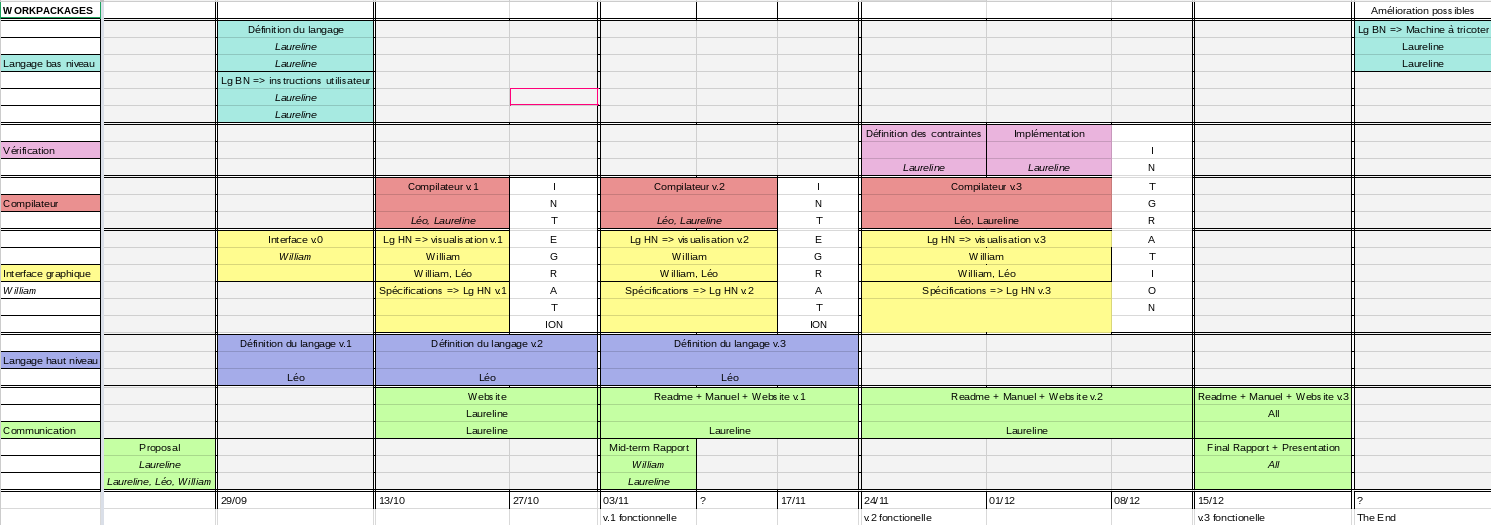
\includegraphics[scale=0.8,angle=270]{calendrier-previsionnel.png}
%  \includegraphics[scale=0.8]{calendrier-previsionnel-part1.png}
%  \includegraphics[scale=0.8]{calendrier-previsionnel-part2.png}
%  \caption{Calendrier prévisionnel des tâches}
%  \label{calendrier}
%\end{figure}

\newpage
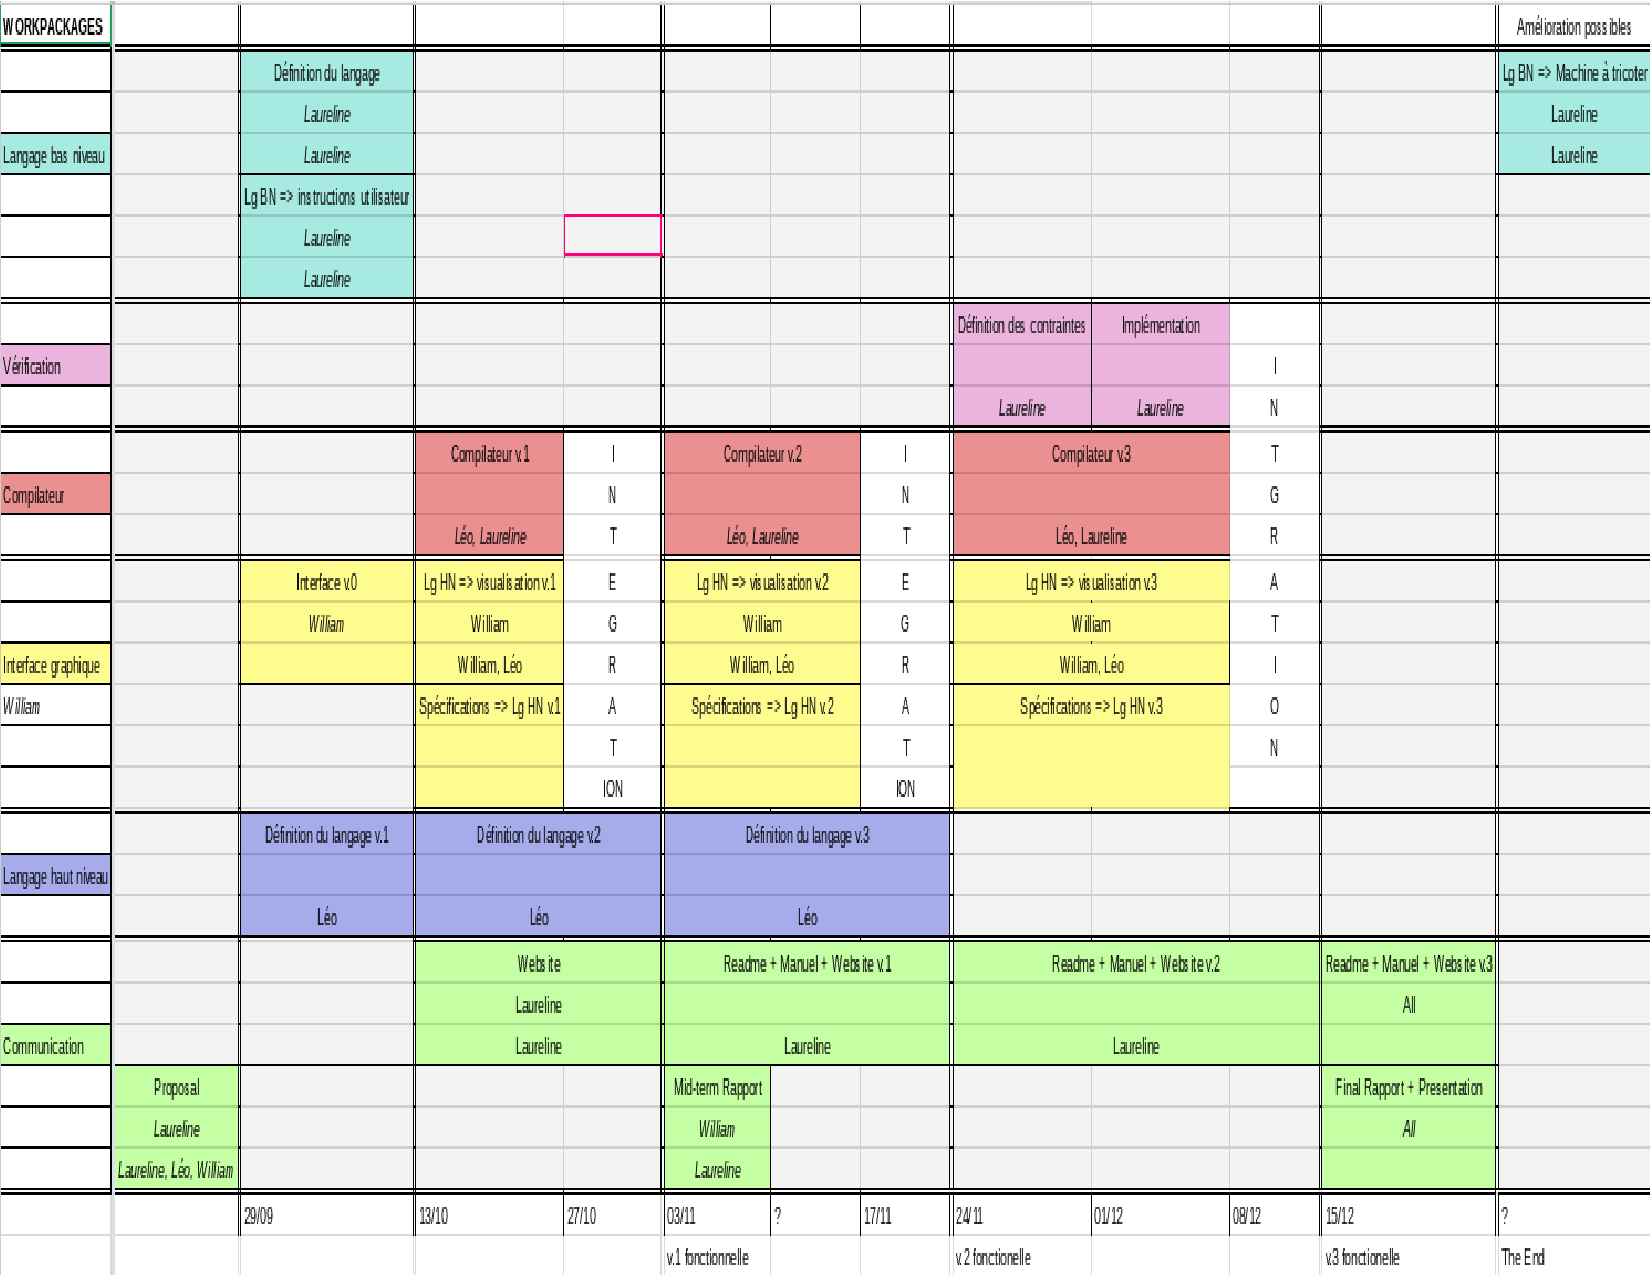
\includepdf{calendrier-previsionnel.pdf} %si on pouvait mettre la page en format paysage ce serait cool

% Calendrier à remplir

\end{document}
